% ===========================================================================
%  İSTANBUL TRAFİK ANOMALİ ANALİZİ — İLERLEME RAPORU
%  Metodoloji, Mimari ve Teknik Gerekçeler
%  Overleaf / pdfLaTeX uyumlu
% ===========================================================================
\documentclass[12pt,a4paper]{article}

% ─── Kodlama ve Dil ───────────────────────────────────────────────────────
\usepackage[utf8]{inputenc}
\usepackage[T1]{fontenc}
\usepackage[turkish]{babel}

% ─── Sayfa Düzeni ─────────────────────────────────────────────────────────
\usepackage{geometry}
\geometry{top=2.5cm, bottom=2.5cm, left=3cm, right=2.5cm}
\usepackage{parskip}
\setlength{\parskip}{6pt}
\setlength{\parindent}{0pt}

% ─── Yazı Tipi ────────────────────────────────────────────────────────────
\usepackage{lmodern}

% ─── Matematik ────────────────────────────────────────────────────────────
\usepackage{amsmath,amssymb,amsthm}

% ─── Tablolar ─────────────────────────────────────────────────────────────
\usepackage{booktabs}
\usepackage{tabularx}
\usepackage{longtable}
\usepackage{array}
\usepackage{float}
\usepackage{graphicx}

% ─── Renk ve Kutu ─────────────────────────────────────────────────────────
\usepackage{xcolor}
\usepackage{tcolorbox}
\tcbuselibrary{skins, breakable}

\definecolor{notebg}{RGB}{235,242,255}
\definecolor{noteframe}{RGB}{50,100,200}
\definecolor{importantbg}{RGB}{255,245,225}
\definecolor{importantframe}{RGB}{200,130,30}
\definecolor{backcolour}{RGB}{248,248,248}
\definecolor{codegreen}{RGB}{40,120,80}
\definecolor{codegray}{RGB}{128,128,128}
\definecolor{codepurple}{RGB}{140,0,180}
\definecolor{codeblue}{RGB}{0,80,180}

% ─── Kod Listeleme ────────────────────────────────────────────────────────
\usepackage{listings}
\lstdefinestyle{codestyle}{
    backgroundcolor=\color{backcolour},
    commentstyle=\color{codegreen}\itshape,
    keywordstyle=\color{codeblue}\bfseries,
    stringstyle=\color{codepurple},
    numberstyle=\tiny\color{codegray},
    basicstyle=\ttfamily\small,
    breakatwhitespace=false,
    breaklines=true,
    captionpos=b,
    keepspaces=true,
    numbers=left,
    numbersep=8pt,
    showspaces=false,
    showstringspaces=false,
    tabsize=2,
    frame=single,
    rulecolor=\color{gray!40},
    xleftmargin=2em,
    framexleftmargin=1.5em,
    aboveskip=8pt,
    belowskip=8pt,
}
\lstset{style=codestyle}

% ─── Notlar / Uyarılar ────────────────────────────────────────────────────
\newtcolorbox{notebox}[1][NOT]{
    enhanced, breakable,
    colback=notebg, colframe=noteframe,
    fonttitle=\bfseries\small, title={#1},
    left=8pt, right=8pt, top=4pt, bottom=4pt,
    before upper={\setlength{\parskip}{4pt}},
}
\newtcolorbox{importantbox}[1][ÖNEMLİ]{
    enhanced, breakable,
    colback=importantbg, colframe=importantframe,
    fonttitle=\bfseries\small, title={#1},
    left=8pt, right=8pt, top=4pt, bottom=4pt,
    before upper={\setlength{\parskip}{4pt}},
}

% ─── Bağlantılar (Hyperref en sona) ───────────────────────────────────────
\usepackage{hyperref}
\hypersetup{
    colorlinks=true,
    linkcolor=blue!60!black,
    urlcolor=blue!60!black,
    citecolor=blue!60!black,
    pdftitle={Istanbul Trafik Anomali Analizi - Ilerleme Raporu},
    pdfauthor={Fikrat Nizamioglu},
}

% ─── Üst-Alt Bilgi ────────────────────────────────────────────────────────
\usepackage{fancyhdr}
\pagestyle{fancy}
\fancyhf{}
\fancyhead[L]{\small\textit{İstanbul Trafik Anomali Analizi — İlerleme Raporu}}
\fancyhead[R]{\small\textit{Fikrat Nizamioğlu}}
\fancyfoot[C]{\small\thepage}
\renewcommand{\headrulewidth}{0.4pt}
\renewcommand{\footrulewidth}{0pt}

% ─── Enumitem ─────────────────────────────────────────────────────────────
\usepackage{enumitem}
\setlist[itemize]{topsep=2pt, itemsep=2pt}
\setlist[enumerate]{topsep=2pt, itemsep=2pt}

% ===========================================================================
\begin{document}

% ─── Kapak ─────────────────────────────────────────────────────────────────
\begin{titlepage}
\centering
\vspace*{3cm}

{\LARGE\bfseries İstanbul Trafik Anomali Analizi}\\[0.6cm]
{\Large İlerleme Raporu}\\[0.3cm]
{\large Metodoloji, Mimari ve Teknik Gerekçeler}\\[2.5cm]

{\normalsize
\begin{tabular}{rl}
\textbf{Proje:}      & İBB Açık Veri Portalı Trafik Yoğunluk Verilerinin \\
                      & PostGIS Tabanlı Mekânsal DBSCAN ve Zamansal Tekrarlanma \\
                      & Analizi ile Anomali Tespiti \\[6pt]
\textbf{Danışman:}    & Dr.\ Mustafa Utku Kalay \\
                      & Yıldız Teknik Üniversitesi \\[6pt]
\textbf{Hazırlayan:}  & Fikrat Nizamioğlu \\[6pt]
\textbf{Tarih:}       & 20 Nisan 2026 \\
\end{tabular}
}
\vfill

{\small
\textit{Bu rapor, projenin mevcut durumunu metodolojik bir çerçevede sunmakta;\\
veri kaynaklarını, algoritmaları, veritabanı tasarımını ve işlem mimarisini\\
teknik gerekçeleriyle birlikte açıklamaktadır.}
}
\end{titlepage}

% ─── İçindekiler ───────────────────────────────────────────────────────────
\tableofcontents
\newpage

\begin{abstract}
Bu rapor, İstanbul Büyükşehir Belediyesi (İBB) Açık Veri Portalı'ndan elde edilen 61 aylık saatlik trafik yoğunluk verisi (Ocak 2020 -- Ocak 2025, 99.628.851 kayıt) üzerinde zaman-uzamsal anomali tespiti gerçekleştiren bir sistemin tasarım ve geliştirme sürecini sunmaktadır. Sistem; PostgreSQL/PostGIS veritabanı altyapısı, PostGIS tabanlı mekânsal DBSCAN kümeleme, zamansal tekrarlılık analizi ve çok kriterli Anomali Yoğunluk Skoru (AIS) hesaplamasından oluşan yedi aşamalı bir boru hattı mimarisi üzerine kurulmuştur. Kümeleme işlemi, PostGIS'in \texttt{ST\_ClusterDBSCAN} pencere fonksiyonu ile EPSG:32636 metreli koordinat sistemi üzerinde veritabanı içinde gerçekleştirilmekte; zamansal boyut ise kümeleme sonrası tekrarlılık ve süre analizi ile değerlendirilmektedir. Bu yaklaşım, tam anlamıyla Birant ve Kut'ın \cite{birant-2007} önerdiği $\epsilon_2$-tabanlı ST-DBSCAN uygulaması değildir; mekânsal DBSCAN ile ardıl zamansal analizin mühendislik düzeyinde bir birleşimidir. 61 aylık tam veri kümesi üzerinde 116 anomali kümesi tespit edilmiş; parametre duyarlılık analizi 192 farklı konfigürasyon üzerinde yürütülmüştür. Sonuçlar FastAPI tabanlı bir REST API aracılığıyla GeoJSON formatında sunulmakta ve Leaflet.js ile etkileşimli harita üzerinde görselleştirilmektedir.
\end{abstract}

% ===========================================================================
\section{Proje Genel Bakışı ve Motivasyon}
% ===========================================================================

Bu çalışma, İstanbul'un taşıt trafiğinde zaman ve mekan boyutunu birlikte ele alarak tekrarlayan tıkanıklık anomalilerini otomatik olarak tespit etmeyi, derecelerini belirlemeyi ve görsel olarak sunmayı amaçlamaktadır. Çalışmanın çıkış noktası, büyük şehirlerde trafik yönetiminin ham veri yoğunluğu karşısında nitelikli karar destek araçlarından yoksun kalmasıdır.

İstanbul genelinde saniyeler içinde değişen trafik koşulları, mevcut manuel yöntemlerle izlenemeyecek düzeyde büyük veri üretmektedir. Bu bağlamda, İBB Açık Veri Portalı'nda kamuyla paylaşılan saatlik trafik yoğunluk veri seti \cite{ibb-portal}, hem yeterliliği hem de erişim kolaylığı bakımından bu çalışma için uygun bir kaynak olarak belirlenmiştir.

Sistem, ham veri yüklenmesinden başlayarak kümeleme analizine, anomali skorlamasına ve nihai görselleştirmeye uzanan tamamen otomatik bir boru hattı (pipeline) üzerine inşa edilmiştir. Her adımda kullanılan teknoloji ve yöntemler, ölçeklenebilirlik, yeniden üretilebilirlik ve akademik geçerlilik ilkeleri gözetilerek seçilmiştir.

% ===========================================================================
\section{Veri Kaynağı: Formatı, İçeriği ve Temin Yöntemi}
% ===========================================================================

\subsection{Kaynağın Belirlenmesi ve Gerekçesi}

İstanbul Büyükşehir Belediyesi, trafik izleme altyapısından elde edilen ham ölçüm verilerini \texttt{data.ibb.gov.tr} adresi üzerinden kamuoyuyla paylaşmaktadır. Bu portal; saatlik trafik yoğunluk verilerini, toplu taşıma verilerini (GTFS formatında) ve değişken kurumsal veri kümelerini bir arada sunmaktadır. Çalışmamızda kullanılan veri kümesi, \textbf{Saatlik Trafik Yoğunluk Veri Seti} adıyla yayımlanan ve aylık periyotlarla güncellenen koleksiyondur.

\begin{importantbox}
Bu çalışmada kullanılan veri, GTFS (General Transit Feed Specification) formatında \textbf{değildir}. GTFS, toplu taşıma güzergâhları için tasarlanmış bir standarttır; bu proje ise araç bazlı trafik yoğunluğunu ölçen ayrı bir listeye dayanmaktadır. Karıştırılmaması gereken kritik bir ayrımdır.
\end{importantbox}

\subsection{Veri Formatı ve Yapısı}

Veri seti, her biri bir aylık dönemi kapsayan \textbf{düz CSV (Comma-Separated Values)} dosyaları biçiminde dağıtılmaktadır. Ocak 2025 dönemi için indirilen dosya yaklaşık 141~MB büyüklüğünde olup 1,7 milyon satır içermektedir.

Her satır, belirli bir coğrafi bölgedeki \textbf{tek bir saatlik ölçümü} temsil etmektedir; dolayısıyla her kayıt kendine özgü bir zaman damgası, bir konum kodu (Geohash) ve o bölgedeki araç davranışını özetleyen istatistikleri barındırmaktadır. Dosya sekiz sütundan oluşmaktadır:

\begin{table}[H]
\centering
\caption{İBB Trafik Yoğunluk CSV Sütun Yapısı}
\label{tab:csv-schema}
\begin{tabularx}{\textwidth}{l l X}
\toprule
\textbf{Sütun Adı} & \textbf{Veri Tipi} & \textbf{Anlamı} \\
\midrule
\texttt{DATE\_TIME}            & Zaman damgası & Ölçümün alındığı kesin an (saatlik granülarite) \\
\texttt{LATITUDE}              & Ondalıklı     & Geohash hücresinin enlem değeri (WGS84, derece) \\
\texttt{LONGITUDE}             & Ondalıklı     & Geohash hücresinin boylam değeri (WGS84, derece) \\
\texttt{GEOHASH}               & Metin         & 6 karakterlik Geohash kodu; yaklaşık 1,2~km $\times$ 0,6~km hücre \\
\texttt{MINIMUM\_SPEED}        & Tamsayı       & O saatte ölçülen en düşük araç hızı (km/h) \\
\texttt{MAXIMUM\_SPEED}        & Tamsayı       & O saatte ölçülen en yüksek araç hızı (km/h) \\
\texttt{AVERAGE\_SPEED}        & Tamsayı       & O saatteki ortalama araç hızı (km/h) \\
\texttt{NUMBER\_OF\_VEHICLES}  & Tamsayı       & O saatte ölçülen toplam araç adedi \\
\bottomrule
\end{tabularx}
\end{table}

\textbf{Geohash nedir ve neden kullanılmıştır?} Geohash, dünya yüzeyini özyinelemeli ızgara hücrelere bölen bir coğrafi kodlama sistemidir. Her hücreye atanan alfanumerik bir kod, hem bölgenin kimliğini hem de konumunu temsil eder. 6 karakterlik bir Geohash kodu yüzey üzerinde yaklaşık $1{,}2 \times 0{,}6$~km'lik bir dikdörtgen alanı ifade eder. İBB'nin bu kodu sütun olarak sunması, aynı coğrafi bölgeyi farklı zaman dilimlerinde gruplamayı kolaylaştırmaktadır.

\subsection{Veri Kümesi Kapsam Özeti}

Bu çalışmada kullanılan veri seti, Ocak 2020 ile Ocak 2025 arasındaki \textbf{61 aylık} dönemi kapsamaktadır. Veri tabanına aktarılan tüm kayıtların özet istatistikleri aşağıdaki tabloda verilmektedir.

\begin{table}[H]
\centering
\caption{İBB Trafik Yoğunluk Veri Kümesi — Genel İstatistikler (61 Ay)}
\label{tab:dataset-summary}
\begin{tabular}{l r}
\toprule
\textbf{Metrik} & \textbf{Değer} \\
\midrule
Toplam satır sayısı    & 99.628.851 \\
Dönem                  & 2020-01-01 -- 2025-01-31 (61 ay) \\
Tekil zaman damgası    & 42.679 \\
Tekil Geohash hücresi  & 5.014 \\
Yinelenen (zaman + geohash) kaydı & 0 \\
Boş (NULL) değerli kayıt & 0 \\
\midrule
Ortalama hız (km/h)    & 56,5 (medyan: 56,0; min: 1; maks: 243) \\
Ortalama araç sayısı   & 79,2 (medyan: 42; min: 1; maks: 2.056) \\
\bottomrule
\end{tabular}
\end{table}

\begin{notebox}[VERİ KALİTESİ NOTLARI]
İki dönemde kaynak-taraflı anomali gözlemlenmiştir; bunlar ingest hatası değil, İBB kaynaklı veri özelliklerinden kaynaklanmaktadır:
\begin{itemize}
    \item \textbf{Ocak 2024:} Yalnızca 957.453 kayıt (tipik ay ortalaması 1,5--1,8~M); İBB veri yayını eksikliği.
    \item \textbf{Haziran 2021:} 5.009 tekil Geohash (diğer aylarda $\sim$2.400); Geohash çözünürlüğü değişikliği.
\end{itemize}
\end{notebox}

\subsection{Verinin Temin Edilme Yöntemi}

Veri, aylık bazda yayımlanan ve sayfalanmamış indirme bağlantılarının dinamik olarak oluşturulduğu bir web arayüzü üzerinden sunulmaktadır. Bu nedenle belediyenin resmi bir API uç noktası yerine, \texttt{requests} ve \texttt{BeautifulSoup} kütüphaneleriyle sistematik bir indirme süreci tasarlanmıştır.

\texttt{download\_data.py} dosyasında yazılan bu süreç şu adımları izlemektedir:

\begin{enumerate}
    \item \textbf{Sayfa Ayrıştırma:} Portal sayfasının HTML içeriği çekilir; \texttt{/download/} veya \texttt{.csv} barındıran tüm bağlantılar tekil hale getirilerek toplanır.
    \item \textbf{Bot Korumasına Karşı Kimlik Bildirimi:} Tüm istekler gerçekçi bir \texttt{User-Agent} başlığıyla gönderilmektedir.
    \item \textbf{Bellek Tasarruflu İndirme:} HTTP akışı, 8~KB'lık parçalar halinde doğrudan diske yazılır.
    \item \textbf{Kesintisiz Devam Desteği:} Daha önce indirilen dosyalar atlanarak işleme kaldığı yerden devam edilir.
\end{enumerate}

\begin{lstlisting}[language=Python, caption={Bellek tasarruflu chunk-download mantığı}]
# stream=True: dosya RAM'e degil, diske parcali olarak yazilir
file_resp = requests.get(link, headers=HEADERS, stream=True)
with open(filepath, 'wb') as f:
    for chunk in file_resp.iter_content(chunk_size=8192):
        if chunk:
            f.write(chunk)
\end{lstlisting}

% ===========================================================================
\section{Veritabanı Tasarımı: PostGIS ve Mekansal Veri Modeli}
% ===========================================================================

\subsection{Teknoloji Seçimi: Neden PostgreSQL/PostGIS?}

Trafik verilerinin depolanmasında ilişkisel bir veritabanı tercih edilmiştir; bunun iki temel gerekçesi vardır.

\textbf{Birincisi}, verinin kendisi doğası gereği ilişkiseldir: her kayıt bir zaman damgası, bir coğrafi konum ve sayısal ölçümlerden oluşur; bu üçlü arasındaki ilişkiyi SQL ifade etmek için tasarlanmıştır.

\textbf{İkincisi ve daha kritik olanı}, standart ilişkisel veritabanlarının coğrafi veriler için özel indeks ve operatör sağlamamasıdır. Bu eksikliği kapatmak amacıyla PostgreSQL üzerine PostGIS uzantısı etkinleştirilmiştir. PostGIS, veritabanına doğrudan nokta, çizgi, çokgen gibi geometri türleri; bu geometriler üzerinde mesafe, kesişim, tampon bölge gibi mekansal sorgular; ve bu sorguları hızlandıran GiST (Generalized Search Tree) mekansal indeks altyapısı kazandırmaktadır \cite{postgis-training}.

Docker üzerinde çalıştırılan konteyner imajı olarak \texttt{mobilitydb/mobilitydb:latest} tercih edilmiştir. MobilityDB \cite{mobilitydb}, PostgreSQL/PostGIS üzerine inşa edilen ve hareketli nesnelerin zamansal geometri sorgularını destekleyen açık kaynaklı bir uzantıdır.

\begin{notebox}[MOBİLİTYDB HAKKINDA]
MobilityDB, Docker imajı aracılığıyla ortamda mevcuttur ve ilerleyen aşamalarda araç yörüngesi analizi gibi geliştirmeler için bir altyapı seçeneği sunmaktadır. Ancak mevcut boru hattında aktif olarak MobilityDB temporal tipi veya fonksiyonu kullanılmamaktadır; kümeleme ve skorlama standart PostgreSQL/PostGIS sorguları ile gerçekleştirilmektedir.
\end{notebox}

\subsection{PostGIS'e Veri Aktarımı: Yöntem ve Gerekçe}

Ham CSV'nin veritabanına aktarılması \texttt{ingest\_data.py} dosyasında kodlanmıştır. Aktarımda \texttt{psycopg2} kütüphanesinin \texttt{execute\_values} fonksiyonu kullanılmıştır.

\begin{notebox}
\texttt{SQL COPY} komutu önceden biçimlendirilmiş, ham sütun değerleri içeren dosyaları satır satır veritabanına aktarmak için idealdir. Ancak bu projede, aktarım sırasında her satırın enlem-boylam çiftinin PostGIS geometri nesnesine dönüştürülmesi gerekmektedir. Bu dönüşüm bir SQL fonksiyonu (\texttt{ST\_MakePoint}) çağrısı gerektirdiğinden, \texttt{COPY} komutu bu senaryo için uygun değildir. \texttt{execute\_values} ise her satır için parametreli SQL şablonu çalıştırma imkânı tanıdığından tercih edilmiştir.
\end{notebox}

Aktarım süreci şu sırayla işlemektedir:

\begin{enumerate}
    \item Bağlantı kurulur ve PostGIS uzantısı aktif değilse \texttt{CREATE EXTENSION IF NOT EXISTS postgis CASCADE} komutuyla etkinleştirilir.
    \item Hedef tablo yoksa \texttt{CREATE TABLE IF NOT EXISTS} ifadesiyle oluşturulur.
    \item CSV dosyası satır satır okunur; eksik veya hatalı sütun barındıran satırlar sessizce atlanır.
    \item Geçerli satırlar 10.000'lik gruplar halinde biriktirilir ve \texttt{execute\_values()} çağrısıyla tek bir SQL yürütmesiyle veritabanına gönderilir.
\end{enumerate}

Geometri oluşturan SQL şablonu aşağıdaki gibidir:

\begin{lstlisting}[language=Python, caption={Geometri oluşturma şablonu}]
ROW_TEMPLATE = (
    "(%s, %s, %s, %s, %s, %s, %s, %s, "
    "ST_SetSRID(ST_MakePoint(%s::double precision,"
    " %s::double precision), 4326))"
)
\end{lstlisting}

Burada \texttt{ST\_MakePoint(lon, lat)} ifadesindeki sıralama dikkat gerektirmektedir: PostGIS ve GeoJSON standardı koordinatları \textbf{(boylam, enlem)} sırasında beklediğinden, CSV'deki sütun sırasından farklı olarak boylam önce verilmektedir.

\subsection{Tablo Şemaları (DDL)}

\subsubsection{Ana Kayıt Tablosu: \texttt{ibb\_traffic\_density}}

Bu tablo, İBB portalından indirilen tüm ham kayıtları saklar. Koordinatlar hem sayısal (sorgulanabilirlik) hem de geometrik (mekansal indeks) biçimde tutulur.

\begin{lstlisting}[language=SQL, caption={Ana veri tablosu DDL}]
CREATE TABLE IF NOT EXISTS ibb_traffic_density (
    id            SERIAL PRIMARY KEY,
    record_time   TIMESTAMP,
    lat           DOUBLE PRECISION,
    lon           DOUBLE PRECISION,
    geohash       VARCHAR(20),
    min_speed     INTEGER,
    max_speed     INTEGER,
    avg_speed     INTEGER,
    vehicle_count INTEGER,
    geom          GEOMETRY(Point, 4326)
);
\end{lstlisting}

\subsubsection{Mekansal İndeks}

PostGIS'in mekansal sorgu performansı, GiST (Generalized Search Tree) tabanlı R-tree indeksine dayanır \cite{crunchy-postgis}. Bu indeks olmadan, bir konumun belli bir yarıçap içindeki komşularını bulmak için tablodaki her satırın mesafesini hesaplamak gerekir. GiST indeksi, yalnızca ilgili coğrafi bölgedeki kayıtlara ulaşarak bu süreci belirgin biçimde hızlandırır.

\begin{lstlisting}[language=SQL, caption={GiST mekansal indeks oluşturma}]
CREATE INDEX IF NOT EXISTS idx_ibb_traffic_geom
ON ibb_traffic_density USING GIST (geom);
\end{lstlisting}

\subsubsection{Ön-Filtreleme Görünümü: \texttt{high\_congestion\_zones}}

Doğrudan ham veri üzerinde kümeleme yapmak hem hesaplama maliyeti hem de anlamsızlık açısından uygun değildir: gece yarısı ıssız bir yolda 15 araçlık düzgün akış, anomali tespitinin dışında kalmalıdır. Bu nedenle analiz öncesinde bir ön eleme aşaması tasarlanmıştır.

\texttt{high\_congestion\_zones} adlı SQL VIEW, \textbf{ortalama hızın 20~km/h'nin altında olduğu} (durma noktasına yakın yavaşlama) ve \textbf{araç sayısının 500'ün üzerinde olduğu} (anlamlı hacim) satırları seçer. 61 aylık tam veri seti üzerinde bu iki koşul birlikte \textbf{9.633 satırlık} bir aday küme oluşturmaktadır (tüm veri setinin \%0,0097'si). Bu eşik değerleri, statik bir temel konfigürasyon olarak benimsenmiştir; parametre duyarlılık analizi farklı eşik kombinasyonlarını Bölüm~\ref{sec:sensitivity} kapsamında incelemektedir.

\begin{lstlisting}[language=SQL, caption={Tıkanıklık ön-filtre görünümü}]
CREATE OR REPLACE VIEW high_congestion_zones AS
SELECT *
FROM ibb_traffic_density
WHERE avg_speed < 20
  AND vehicle_count > 500;
\end{lstlisting}

\subsubsection{Sonuç Tablosu: \texttt{traffic\_clusters}}

Kümeleme boru hattının çıktısı bu tabloya yazılır. Her kayıt hangi anomali kümesine ait olduğunu belirten \texttt{cluster\_id} sütununu, AIS skorunu ve şiddet sınıfını içermektedir.

\begin{lstlisting}[language=SQL, caption={Kümeleme sonuç tablosu DDL}]
CREATE TABLE IF NOT EXISTS traffic_clusters (
    id            SERIAL PRIMARY KEY,
    record_time   TIMESTAMP WITHOUT TIME ZONE,
    lat           DOUBLE PRECISION,
    lon           DOUBLE PRECISION,
    geohash       VARCHAR(20),
    vehicle_count INTEGER,
    avg_speed     INTEGER,
    cluster_id    INTEGER,   -- PostGIS ST_ClusterDBSCAN etiketi; -1 = gurultu
    ais_score     NUMERIC(5,4),
    severity      VARCHAR(10)
);
\end{lstlisting}

\subsection{Koordinat Referans Sistemi: EPSG:4326 Aktarım, EPSG:32636 Kümeleme}

İBB kaynaklı CSV koordinatları \textbf{WGS84 (EPSG:4326)} coğrafi koordinatlarıdır ve bu biçimde veritabanına aktarılmaktadır. Ancak mesafe tabanlı kümeleme için düzlemsel bir projeksiyon zorunludur.

\textbf{Neden EPSG:32636?} PostGIS'in \texttt{ST\_ClusterDBSCAN} fonksiyonunun \texttt{eps} (yarıçap) parametresi, geometrinin doğal birimini kullanır. EPSG:4326 ile bu birim derecedir; bir derece $\approx 111$~km'ye karşılık geldiğinden, gerçek metre cinsinden mesafe ifadesi mümkün değildir. EPSG:32636 (UTM Zone 36N), İstanbul'u kapsayan ve metreyi doğal birim olarak kullanan bir düzlemsel koordinat sistemidir. Bu projeksiyon seçimi sayesinde \texttt{eps = 500} ifadesi doğrudan 500~metre anlamına gelir.

Koordinat dönüşümü kümeleme aşamasında SQL içinde gerçekleştirilmektedir:

\begin{lstlisting}[language=SQL, caption={EPSG:4326 -> EPSG:32636 dönüşümü ve ST\_ClusterDBSCAN}]
SELECT
    geohash,
    avg_speed,
    vehicle_count,
    ST_ClusterDBSCAN(
        ST_Transform(geom, 32636),
        eps := 500,
        minpoints := 3
    ) OVER () AS cluster_id
FROM high_congestion_zones;
\end{lstlisting}

\begin{notebox}
Eğer veri aktarımı aşamasında tablo, WGS84 (EPSG:4326) geometrisi ile oluşturulmuşsa, kümeleme sırasında \texttt{ST\_Transform(geom, 32636)} çağrısı ile koordinatlar çalışma zamanında EPSG:32636'ya dönüştürülür. Bu dönüşüm, kaynak verisinin orijinal koordinatlarını bozmadan mesafe hesaplamalarının metre cinsinden yapılmasını sağlar.
\end{notebox}

% ===========================================================================
\section{Kümeleme Metodolojisi: PostGIS Tabanlı Mekânsal DBSCAN}
% ===========================================================================

\subsection{Yöntem Seçimi ve Kavramsal Çerçeve}

Bu projede kümeleme yöntemi, üç temel alternatifin değerlendirilmesiyle belirlenmiştir:

\begin{table}[H]
\centering
\caption{Kümeleme Yöntemi Karşılaştırması}
\label{tab:method-comparison}
\begin{tabularx}{\textwidth}{l X c}
\toprule
\textbf{Yöntem} & \textbf{Tanım} & \textbf{Bu projede?} \\
\midrule
DBSCAN & Yoğunluk tabanlı mekânsal kümeleme; tek $\epsilon$ ile komşuluk tanımlar & Kavramsal zemin \\
ST-DBSCAN \cite{birant-2007} & Hem mekânsal ($\epsilon_1$) hem de zamansal ($\epsilon_2$) komşuluk kısıtı; iki epsilon ile tam zaman-uzamsal kümeleme & Tam olarak uygulanmadı \\
PostGIS \texttt{ST\_ClusterDBSCAN} & PostgreSQL pencere fonksiyonu; geometriler üzerinde mekânsal DBSCAN & \textbf{Evet, aktif kullanım} \\
\midrule
\textbf{Bu projenin yaklaşımı} & Mekânsal DBSCAN (PostGIS) + kümeleme sonrası zamansal tekrarlılık/süre analizi + AIS skorlama & \textbf{Evet} \\
\bottomrule
\end{tabularx}
\end{table}

\begin{importantbox}[METODOLOJİ AÇIKLAMASI]
Bu proje, Birant ve Kut'ın \cite{birant-2007} önerdiği $\epsilon_2$ tabanlı zamansal komşuluk kısıtını doğrudan uygulamamaktadır. Zamansal boyut, kümeleme sonrasında ayrı bir analiz adımında değerlendirilmektedir: küme kayıtlarının kaç farklı güne ve saate yayıldığı (tekrarlılık ve süre) AIS skorunun bileşenleri olarak hesaplanmaktadır. Bu, ST-DBSCAN fikrinin mühendislik düzeyinde bir uyarlamasıdır, tam bir $\epsilon_2$-tabanlı ST-DBSCAN uygulaması değildir.
\end{importantbox}

\subsection{PostGIS \texttt{ST\_ClusterDBSCAN} Tercihinin Gerekçesi}

Python tabanlı bir BallTree + DBSCAN uygulaması yerine PostGIS \texttt{ST\_ClusterDBSCAN}'ın tercih edilmesinin üç somut gerekçesi vardır:

\textbf{1. Veri hareketini ortadan kaldırma:} 9.633 satırlık aday kümenin veritabanından Python'a aktarılması, ardından geri yazılması gereksiz I/O yüküne yol açar. PostGIS, bu hesaplamayı veri yerinde gerçekleştirir.

\textbf{2. Mekansal indeks entegrasyonu:} \texttt{ST\_ClusterDBSCAN}, GiST indeksini doğrudan kullanarak komşuluk sorgularını tam tablo taramasız yanıtlar.

\textbf{3. Basit çalışma süresi:} 61 aylık tam veri setinde (9.633 aday nokta) kümeleme 3,66~saniyede tamamlanmaktadır. Bu, uygulama karmaşıklığını artırmadan yeterli performans sunmaktadır.

\subsection{Parametre Konfigürasyonu}

\begin{table}[H]
\centering
\caption{PostGIS ST\_ClusterDBSCAN Parametre Konfigürasyonu (Temel)}
\label{tab:dbscan-params}
\begin{tabular}{l l l}
\toprule
\textbf{Parametre} & \textbf{Değer} & \textbf{Gerekçe} \\
\midrule
\texttt{eps}       & 500~m  & Tek bir İstanbul kavşak/kesişim bölgesini kapsayan mesafe; EPSG:32636 metre birimi \\
\texttt{minpoints} & 3      & Az sayıda noktadan oluşan gerçek anomalileri yakalayan asgari eşik \\
\bottomrule
\end{tabular}
\end{table}

\texttt{eps = 500}~m değeri, İstanbul'un yoğun kavşak yapısında tek bir trafik düğümünü kapsayacak, ancak birden fazla bağımsız kavşağı birleştirmeyecek ölçekte seçilmiştir. Parametre kısıtları ve bunların küme sayısına, gürültü oranına ve çalışma süresine etkisi Bölüm~\ref{sec:sensitivity} içinde sistematik biçimde incelenmektedir.

\subsection{Zamansal Tekrarlılık Analizi}

PostGIS kümeleme yalnızca mekânsal komşuluğu değerlendirir. Zamansal boyut, küme ataması tamamlandıktan sonra her küme için aşağıdaki istatistikler hesaplanarak AIS bileşenlerine dahil edilir:

\begin{itemize}
    \item \textbf{Süre (Duration):} Küme içindeki en erken ve en geç kayıt zaman damgası arasındaki saat farkı.
    \item \textbf{Tekrarlılık (Recurrence):} Küme kayıtlarının kaç farklı takvim gününe yayıldığı.
\end{itemize}

Bu iki boyut, uzun süreli ve sık tekrarlayan tıkanıklıkları kısa süreli olaylardan ayırt etmek amacıyla AIS formülünde ağırlıklı olarak değerlendirilmektedir (bkz. Bölüm~\ref{sec:ais}).

\subsection{Tam Veri Seti Sonuçları}

61 aylık tam veri seti üzerinde (9.633 aday nokta, temel parametre konfigürasyonu) elde edilen sonuçlar:

\begin{table}[H]
\centering
\caption{Kümeleme Sonuçları — Tam Veri Seti (61 Ay, 2020--2025)}
\label{tab:cluster-results}
\begin{tabular}{l r}
\toprule
\textbf{Metrik} & \textbf{Değer} \\
\midrule
Aday nokta sayısı (ön-filtreden sonra) & 9.633 \\
Oluşturulan küme sayısı & 116 \\
Gürültü (noise) noktası sayısı & 78 \\
Gürültü oranı & \%0,81 \\
Kümeleme çalışma süresi & 3,66~s \\
\midrule
AIS aralığı & 0,044 -- 0,769 \\
AIS ortalaması & 0,347 \\
\midrule
HIGH (\%66 üzeri) küme sayısı & 3 \\
MEDIUM (\%33--\%66) küme sayısı & 59 \\
LOW (\%33 altı) küme sayısı & 54 \\
\bottomrule
\end{tabular}
\end{table}

% ===========================================================================
\section{Dinamik Yoğunluk Filtreleme}
% ===========================================================================

\subsection{Statik Filtre Sınırlılıkları}

Bölüm~\ref{sec:db}'de tanımlanan statik filtre (\texttt{avg\_speed < 20 AND vehicle\_count > 500}) sabit eşik değerlerine dayanır ve coğrafi bağlamı göz ardı eder. İstanbul'un farklı bölgelerinde yol yapısı ve kapasitesi büyük ölçüde değiştiğinden, aynı araç yoğunluğu dar bir mahalle sokağında gerçek bir tıkanıklığa işaret ederken geniş bir ana arter için normal kabul edilebilir.

Bu kısıtlamayı ele almak amacıyla iki ek filtreleme yaklaşımı prototip düzeyinde geliştirilmiş ve karşılaştırmalı olarak değerlendirilmiştir.

\subsection{Geohash Alan Yoğunluğu Prototipi}

\textbf{Yaklaşım:} Her Geohash hücresinin yüzey alanı (km²) hesaplanarak araç yoğunluğu birimine (araç/km²) dönüştürülür. Bu değer üzerinden percentil tabanlı bir yoğunluk eşiği belirlenir.

\begin{lstlisting}[language=SQL, caption={Geohash alan yoğunluğu hesaplama (prototip)}]
-- Geohash hucre alani EPSG:32636 uzerine donusturulmus
-- geometri ile hesaplanir (metre karesi -> km kare)
SELECT
    geohash,
    AVG(vehicle_count)            AS avg_vehicle_count,
    ST_Area(ST_Transform(
        ST_Envelope(ST_Collect(geom)), 32636
    )) / 1e6                      AS cell_area_km2,
    AVG(vehicle_count) / (
        ST_Area(ST_Transform(
            ST_Envelope(ST_Collect(geom)), 32636
        )) / 1e6
    )                             AS vehicles_per_km2
FROM ibb_traffic_density
GROUP BY geohash;
\end{lstlisting}

\begin{importantbox}[SINIRLILIK]
Bu yaklaşım, bir yüzey alanı yaklaşımıdır. Araç sayısı, Geohash hücresindeki toplam yol uzunluğuna değil, hücrenin tahmini yüzey alanına bölünmektedir. Gerçek yol ağı verisi kullanılmadan elde edilen bu değer, yol yoğunluğunu temsil etmemektedir. Bu nedenle sonuçlar bir ön araştırma prototipi olarak değerlendirilmeli; kesin trafik yoğunluk ölçütü olarak kullanılmamalıdır.
\end{importantbox}

Prototip sonuçları: 75. percentil eşiği ($\geq 270{,}81$~araç/km², en az 50~araç koşuluyla) uygulandığında:

\begin{table}[H]
\centering
\caption{Statik Filtre ile Geohash Alan Yoğunluğu Karşılaştırması}
\label{tab:density-comparison}
\begin{tabular}{l r r r}
\toprule
\textbf{Metrik} & \textbf{Statik} & \textbf{Alan Yoğunluğu} & \textbf{Kesişim} \\
\midrule
Seçilen geohash sayısı & 174 & 333 & 157 \\
Yalnızca bu yöntemde  & 17 & 176 & — \\
\bottomrule
\end{tabular}
\end{table}

\begin{figure}[H]
\centering
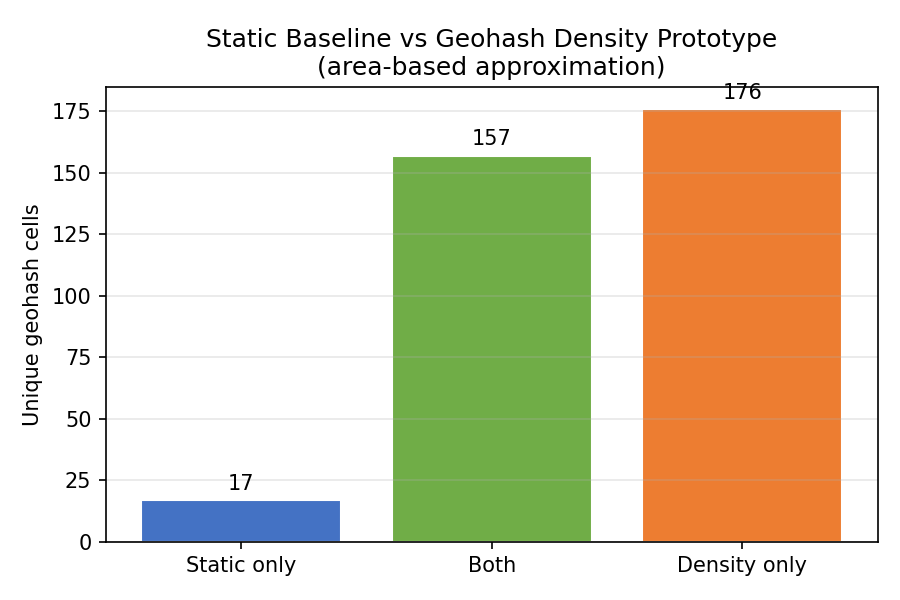
\includegraphics[width=0.95\textwidth]{figures/experiments/density_filter_comparison}
\caption{Statik filtre ile geohash-alan yoğunluğu filtresinin karşılaştırılması}
\label{fig:density-comparison}
\end{figure}

\subsection{Yol Ağı Tabanlı Yoğunluk Analizi}

\textbf{Yaklaşım:} OpenStreetMap (OSM) verisi PostGIS'e aktarılarak her Geohash hücresiyle çakışan yol segmentlerinin toplam uzunluğu hesaplanır. Araç yoğunluğu bu uzunluğa (araç/yol-km) bölünerek yol ağı farkındaki bir yoğunluk skoru elde edilir.

\begin{lstlisting}[language=SQL, caption={Yol ağı tabanlı yoğunluk (PostGIS + OSM)}]
SELECT
    g.geohash,
    SUM(ST_Length(
        ST_Intersection(r.geom, ST_Transform(g.cell_geom, 32636))
    )) / 1000.0   AS road_km,
    g.avg_vehicles / (
        SUM(ST_Length(
            ST_Intersection(r.geom, ST_Transform(g.cell_geom, 32636))
        )) / 1000.0
    )             AS vehicles_per_road_km
FROM geohash_cells g
JOIN osm_roads r
  ON ST_Intersects(r.geom, ST_Transform(g.cell_geom, 32636))
GROUP BY g.geohash, g.avg_vehicles;
\end{lstlisting}

OSM veri seti ve yol ağı analizi sonuçları:

\begin{table}[H]
\centering
\caption{Yol Ağı Tabanlı Yoğunluk Analizi Sonuçları}
\label{tab:road-density}
\begin{tabular}{l r}
\toprule
\textbf{Metrik} & \textbf{Değer} \\
\midrule
OSM yol segmenti sayısı    & 126.044 \\
Toplam yol ağı uzunluğu    & 16.151,3~km \\
Yol kapsayan Geohash hücresi & 1.583 / 5.014 (\%31,6) \\
Yol kapsama alanı dışı kayıt & 34.375.270 (\%34,5 / veri seti) \\
Yol yoğunluğu eşiği (p75) & 15,73~araç/yol-km \\
\midrule
Statik filtre seçimi (geohash) & 174 \\
Yol yoğunluğu seçimi (geohash) & 397 \\
Kesişim (her iki yöntemde)     & 99 \\
Yalnızca statik              & 75 \\
Yalnızca yol yoğunluğu       & 298 \\
\bottomrule
\end{tabular}
\end{table}

\begin{notebox}
Veri setinin \%34,5'i yol ağı kapsama alanı dışında kalan Geohash hücrelerine aittir. Bu hücrelerin araç yoğunluğu hesaplanamaz; dolayısıyla yol ağı tabanlı filtreleme bu kayıtları değerlendirememektedir. Bu durum, yol ağı yoğunluk yaklaşımının statik filtreye göre daha seçici olduğu bazı bölgelerde eksik kapsama yaratabileceğini göstermektedir. \texttt{sxk8xg} geohash'i gibi aşırı uç değerler (31.859~araç/yol-km, 0,002~km yol) mevcut OSM verisindeki kısa yol segmenti artifaktlarına işaret etmekte ve filtreleme öncesi temizlenmelidir.
\end{notebox}

\begin{figure}[H]
\centering
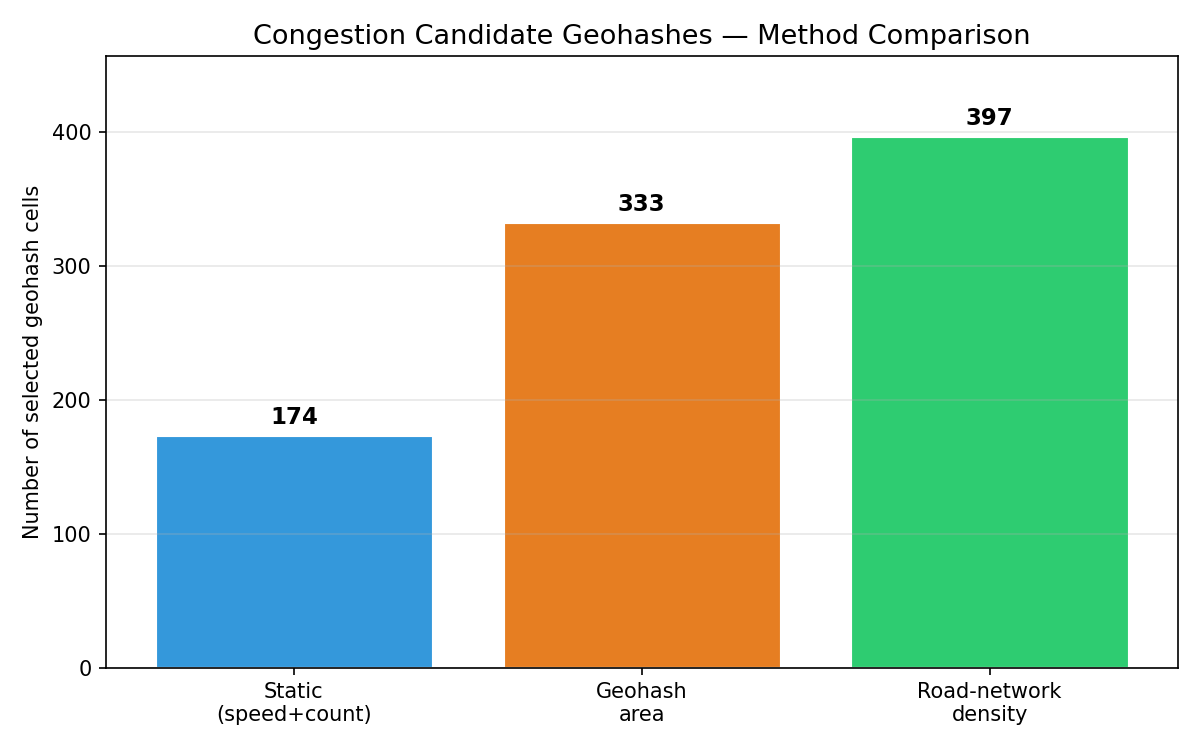
\includegraphics[width=0.95\textwidth]{figures/experiments/road_density_filter_comparison}
\caption{Statik filtre ile yol ağına duyarlı yoğunluk filtresinin karşılaştırılması}
\label{fig:road-density}
\end{figure}

% ===========================================================================
\section{İşlem Yükü Dağılımı: PostGIS İçinde mi, Python Dışında mı?}
% ===========================================================================

Projenin bileşenleri arasındaki iş bölümü, her katmanın güçlü yönlerinden yararlanan \textbf{hibrit bir mimari} çerçevesinde düzenlenmiştir.

\subsection{PostGIS'e Bırakılan Sorumluluklar}

\begin{itemize}
    \item \textbf{Geometri oluşturma ve depolama:} Her satırın koordinatları, aktarım anında SQL düzeyinde \texttt{ST\_MakePoint()} ile PostGIS Point nesnesine dönüştürülür.
    \item \textbf{Mekansal indeksleme:} GiST tabanlı R-tree indeksi, bölgesel mekansal sorguları tam tablo taramasız yanıtlar.
    \item \textbf{Ön-filtreleme:} \texttt{high\_congestion\_zones} VIEW, veriyi 99,6~M kayıttan 9.633 adaya indirir.
    \item \textbf{Mekânsal DBSCAN kümeleme:} \texttt{ST\_ClusterDBSCAN} fonksiyonu, EPSG:32636 üzerinde veri yerinde çalışır.
    \item \textbf{Küme istatistikleri:} FastAPI katmanı, küme merkezlerini, ortalama metrikleri ve zirve zamanlarını SQL üzerinden hesaplar.
    \item \textbf{Yol ağı analizi:} OSM yol segmentleriyle kesişim hesapları PostGIS geometri fonksiyonlarıyla (\texttt{ST\_Length}, \texttt{ST\_Intersection}, \texttt{ST\_Intersects}) veritabanı içinde yürütülür.
\end{itemize}

\subsection{Python'a Bırakılan Sorumluluklar}

\begin{itemize}
    \item \textbf{Anomali Şiddet Skorlaması (AIS):} Dört bileşenin min-max normalizasyonu ve ağırlıklı toplamı Pandas DataFrame üzerinde \texttt{scoring/anomaly\_score.py} içinde vektörel olarak hesaplanır.
    \item \textbf{Parametre duyarlılık deneyleri:} Farklı $\{\text{hız eşiği}, \text{araç eşiği}, \text{eps}, \text{minpoints}\}$ kombinasyonlarının taranması Python orkestrasyon mantığıyla yürütülür.
    \item \textbf{Raporlama ve görselleştirme:} CSV, Markdown ve PNG çıktıları Python betikleriyle üretilir.
\end{itemize}

\subsection{Veri Akışının Özeti}

\begin{lstlisting}[language={}, numbers=none, caption={Hibrit mimarinin veri akisi}]
1. PostGIS  -> high_congestion_zones VIEW (SQL filtre: 9.633 aday)
2. PostGIS  -> ST_ClusterDBSCAN EPSG:32636 uzerinde (116 kume, 78 gurultu)
3. Python   -> AIS skorlama (scoring/anomaly_score.py)
4. PostGIS  -> execute_values() ile traffic_clusters'a geri yazma
5. PostGIS  -> FastAPI SQL sorgulariyla GeoJSON donusturme
6. Python   -> Leaflet.js'e REST API ile servis etme
\end{lstlisting}

% ===========================================================================
\section{Anomali Şiddet Skorlaması (AIS)}
\label{sec:ais}
% ===========================================================================

\subsection{Metodolojik Gerekçe}

Kümeleme yalnızca hangi noktaların birlikte gruplanabileceğini söyler; hangi kümenin daha kritik olduğuna ilişkin bir hiyerarşi kurmaz. Bu eksikliği gidermek için \textbf{Çok Kriterli Karar Analizi (MCDA — Multi-Criteria Decision Analysis)} metodolojisine dayanan özel bir Anomali Şiddet Skoru (AIS) geliştirilmiştir.

\subsection{Bileşenler ve Formül}

\begin{equation}
\text{AIS}(C_k) = w_1 \hat{V}_k + w_2 \hat{S}_k + w_3 \hat{D}_k + w_4 \hat{R}_k
\label{eq:ais}
\end{equation}

\begin{table}[H]
\centering
\caption{AIS Bileşenleri, Hesaplanışları ve Ağırlıkları}
\label{tab:ais-components}
\begin{tabularx}{\textwidth}{c l X c}
\toprule
\textbf{Sem.} & \textbf{Bileşen} & \textbf{Ham değer \& hesaplama} & \textbf{Ağırlık ($w$)} \\
\midrule
$\hat{V}$ & Volume (Hacim) &
    Kümedeki ortalama araç sayısı; daha fazla araç = daha ciddi tıkanıklık &
    0,30 \\
$\hat{S}$ & Speed Drop (Hız Düşüşü) &
    $1 - (\bar{v}_k / v_{\text{city}})$; kentsel referans hız 35~km/h.\ Hız sıfıra ne kadar yakınsa değer o kadar büyük.\ $[0,1]$'e kırpılır. &
    0,30 \\
$\hat{D}$ & Duration (Süreklilik) &
    Kümedeki en geç ve en erken kayıt farkı (saat cinsinden). Uzun süreli tıkanıklık daha ciddi. &
    0,25 \\
$\hat{R}$ & Recurrence (Tekrarlama) &
    Küme kayıtlarının kaç farklı takvim gününe ait olduğu. Birden fazla günde tekrarlayan anomali altyapısal sorun işareti. &
    0,15 \\
\bottomrule
\end{tabularx}
\end{table}

Her bileşen \textbf{min-max normalizasyonuyla} $[0, 1]$ aralığına getirilir:

\begin{equation}
\hat{x} = \frac{x - x_{\min}}{x_{\max} - x_{\min}}
\label{eq:minmax}
\end{equation}

Normalizasyon, tüm kümeler arasında görece sıralama korur. Eğer tüm kümeler aynı değere sahipse (bölücü sıfır) bileşen 0,5 olarak sabitlenir.

\subsection{Sınıflandırma}

Birleşik AIS skoru üç seviyeli bir alarm sınıfına atanır:

\begin{equation}
\text{Severity}(C_k) =
\begin{cases}
\textbf{HIGH}   & \text{AIS} \in [0{,}66,\; 1{,}00] \\
\textbf{MEDIUM} & \text{AIS} \in [0{,}33,\; 0{,}66) \\
\textbf{LOW}    & \text{AIS} \in [0{,}00,\; 0{,}33)
\end{cases}
\end{equation}

\subsection{Tam Veri Seti Üzerindeki Sonuçlar}

61 aylık tam veri seti üzerinde çalıştırılan boru hattı 116 anomali kümesi tespit etmiş ve aşağıdaki dağılım elde edilmiştir:

\begin{table}[H]
\centering
\caption{AIS Skorlama Sonuçları — Tam Veri Seti (61 Ay, 116 Küme)}
\label{tab:ais-results}
\begin{tabular}{l r r r}
\toprule
\textbf{Şiddet Sınıfı} & \textbf{AIS Aralığı} & \textbf{Küme Sayısı} & \textbf{Oran} \\
\midrule
HIGH   & 0,66 -- 0,769 & 3  & \%2,6  \\
MEDIUM & 0,33 -- 0,659 & 59 & \%50,9 \\
LOW    & 0,044 -- 0,329 & 54 & \%46,6 \\
\midrule
\textbf{Toplam} & 0,044 -- 0,769 & \textbf{116} & \%100 \\
\bottomrule
\end{tabular}
\end{table}

AIS ortalaması 0,347 olup kümelerin çoğunluğunun MEDIUM kategorisinde yer aldığını göstermektedir. HIGH kategorisindeki 3 küme, 20~km/h'nin altında süregelen hız ve 500'ün üzerinde araç yoğunluğu ile yüksek tekrarlılık gösteren konumlara karşılık gelmektedir. Bu bulgular, söz konusu noktaların anlık değil yapısal tıkanıklık bölgeleri olduğuna işaret etmektedir.

Gürültü noktaları (cluster\_id = $-1$): 78 nokta, toplam aday setinin \%0,81'i; bunlar yeterli komşu yoğunluğuna sahip olmayan izole kayıtlardır.

% ===========================================================================
\section{Parametre Duyarlılık Analizi}
\label{sec:sensitivity}
% ===========================================================================

Danışman değerlendirmesi, parametre seçiminin gerekçelendirilmesi gereken bir metodoloji açığı olarak not edilmiştir. Bu gerekliliği karşılamak amacıyla \texttt{experiments/parameter\_sensitivity.py} betiği 192 farklı parametre kombinasyonunu sistematik biçimde test etmiştir.

\subsection{Deney Tasarımı}

Test edilen parametre uzayı:

\begin{table}[H]
\centering
\caption{Parametre Duyarlılık Deney Tasarımı}
\label{tab:sensitivity-grid}
\begin{tabular}{l l}
\toprule
\textbf{Parametre} & \textbf{Test Edilen Değerler} \\
\midrule
Hız eşiği (km/h)       & 10, 15, 20, 25 \\
Araç sayısı eşiği      & 300, 500, 700, 1000 \\
\texttt{eps} (metre)   & 250, 500, 750, 1000 \\
\texttt{minpoints}     & 3, 5, 10 \\
\midrule
Toplam kombinasyon & $4 \times 4 \times 4 \times 3 = 192$ \\
Toplam çalışma süresi & 468,5~s \\
\bottomrule
\end{tabular}
\end{table}

\subsection{Temel Bulgular}

\begin{itemize}
    \item \textbf{Sıfır küme üretilen konfigürasyonlar:} 64 kombinasyon hiç küme üretememiştir. Bu durum \texttt{hız = 10} içeren tüm konfigürasyonlarda ve \texttt{hız = 15, araç $\geq$ 1000} konfigürasyonlarında ortaya çıkmaktadır. 10~km/h eşiği, ön-filtreye giren aday noktası sayısını DBSCAN için yeterli yoğunluk oluşturmayacak kadar düşürmektedir.

    \item \textbf{Temel konfigürasyon} (hız=20, araç=500, eps=500, minpoints=3): 9.633 aday $\to$ 116 küme, \%0,81 gürültü. Bu değerler, anlamlı küme sayısı ile kabul edilebilir gürültü oranını dengeli biçimde sağlamaktadır.

    \item \textbf{En gevşek konfigürasyon} (hız=25, araç=300, eps=250, minpoints=3): 222.295 aday $\to$ 515 küme; çalışma süresi 11--39~s arasında artmaktadır. Bu konfigürasyonda küme sayısının yüksekliği ve gürültü oranının düşüklüğü (\%0,07), birçok küçük ve muhtemelen önemsiz grubun küme olarak kabul edildiğine işaret etmektedir.

    \item \textbf{\texttt{eps} etkisi:} \texttt{eps = 1000}~m kullanıldığında temel konfigürasyondaki 116 küme 39 kümeye düşmektedir; geniş yarıçap birbirinden bağımsız bölgeleri birleştirmektedir. Bu gözlem, 500~m seçiminin İstanbul kavşak ölçeğiyle daha iyi örtüştüğünü desteklemektedir.
\end{itemize}

\begin{figure}[H]
\centering
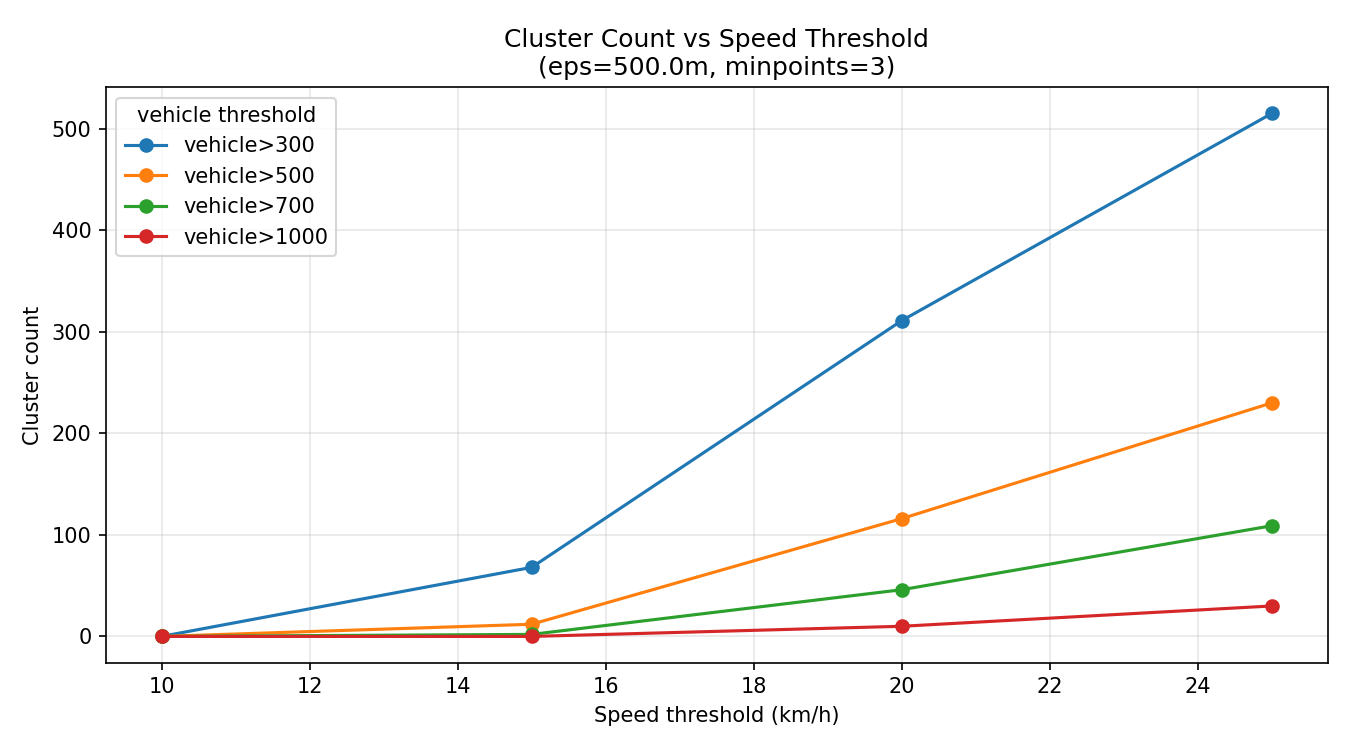
\includegraphics[width=0.95\textwidth]{figures/experiments/threshold_impact}
\caption{Hız ve araç eşiklerinin küme sayısına etkisi}
\label{fig:threshold-impact}
\end{figure}

\begin{figure}[H]
\centering
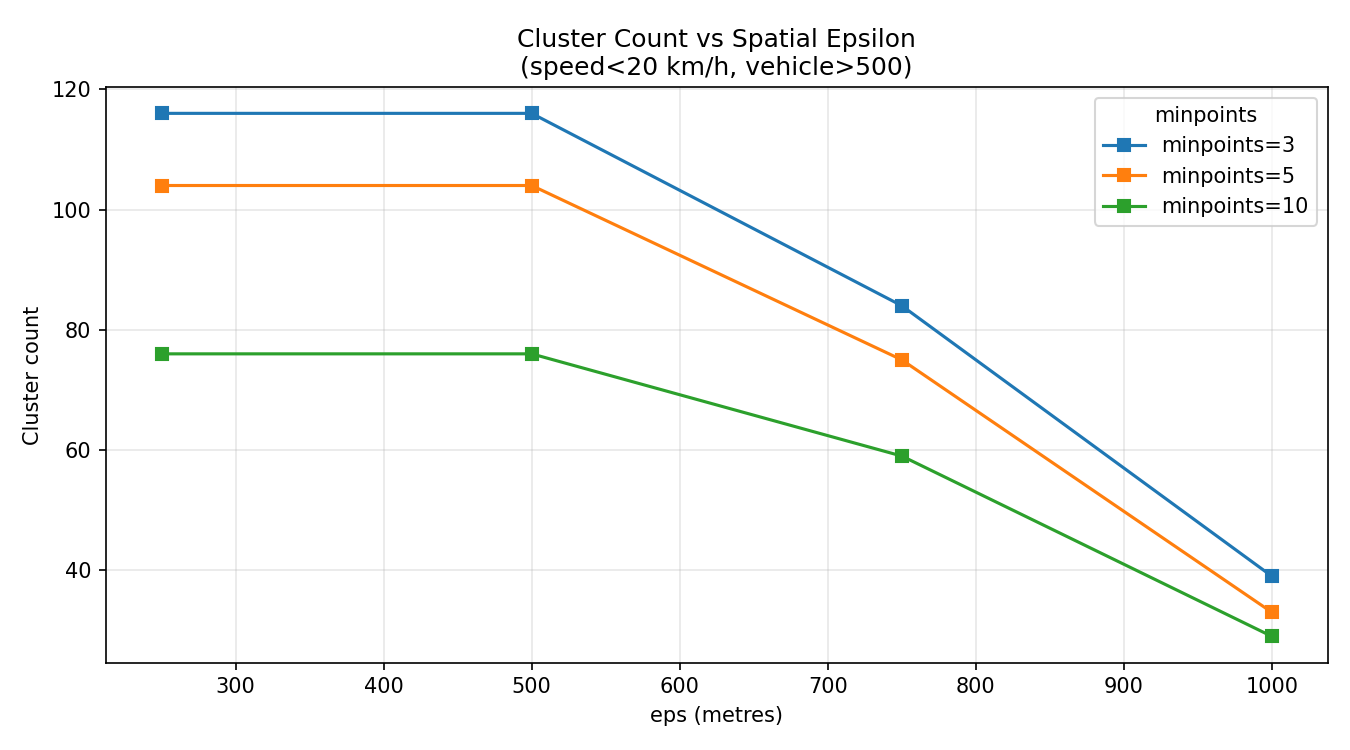
\includegraphics[width=0.95\textwidth]{figures/experiments/eps_minpoints_impact}
\caption{eps ve minpoints parametrelerinin karşılaştırılması}
\label{fig:eps-minpoints}
\end{figure}

\begin{figure}[H]
\centering
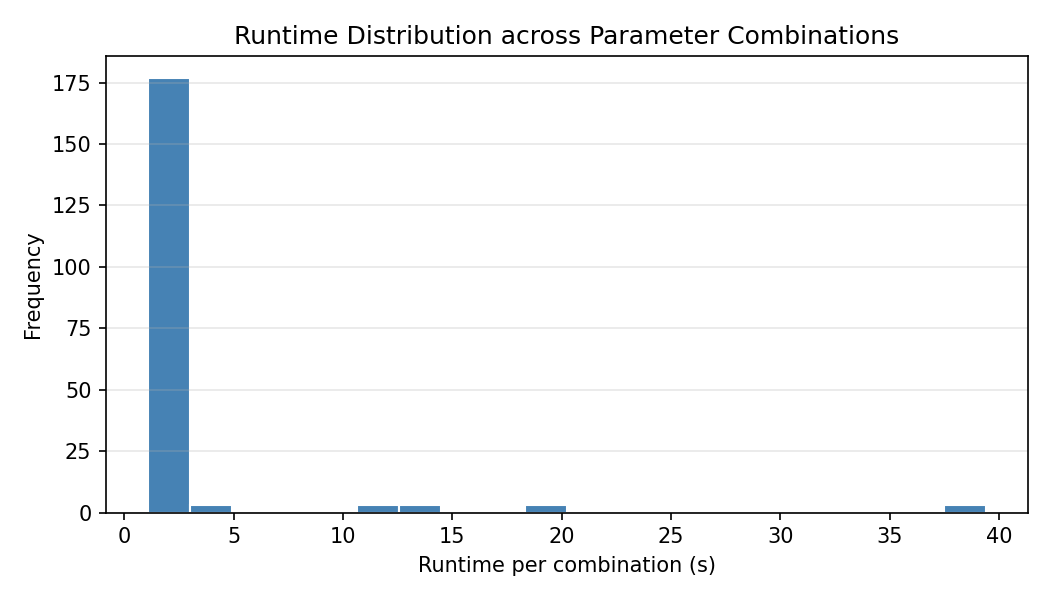
\includegraphics[width=0.95\textwidth]{figures/experiments/runtime_comparison}
\caption{Parametre konfigürasyonlarına göre çalışma süresi dağılımı}
\label{fig:runtime}
\end{figure}

% ===========================================================================
\section{Küme Doğrulama}
% ===========================================================================

Kümeleme sonuçlarının kalitesini değerlendirmek için niceliksel metrik hesaplamak yerine, bu çalışmada \textbf{konfigürasyon karşılaştırması} ve \textbf{çıktı analizi} yöntemi benimsenmiştir. Bunun nedeni, yoğunluk tabanlı kümeleme doğrulama metriklerinin (Silhouette Skoru, Davies-Bouldin İndeksi) standart Öklid mesafesini baz alması ve ST tabanlı veriler için doğrudan yorumlanamamasıdır.

Kullanılan doğrulama yaklaşımları şunlardır:

\begin{enumerate}
    \item \textbf{Gürültü oranı izleme:} Temel konfigürasyonda \%0,81 gürültü oranı, aday noktaların büyük çoğunluğunun kümeye dahil edildiğini göstermektedir. Gürültü oranı hem çok düşük (aşırı kümeleme) hem de çok yüksek (yetersiz kümeleme) konfigürasyonları belirlememizi sağlamaktadır.

    \item \textbf{Küme sayısı tutarlılığı:} 192 kombinasyon üzerinde küme sayısının 0 ile 515 arasında değişmesi, parametre uzayının kapsayıcı biçimde tarandığını ve seçilen temel konfigürasyonun (116 küme) bu aralığın ortasına denk geldiğini göstermektedir.

    \item \textbf{AIS skor dağılımı:} 116 küme içinde HIGH:3, MEDIUM:59, LOW:54 dağılımı, sistemin küme havuzunu anlamlı biçimde ayrıştırdığını; tüm kümeler aynı kategoriye yığılmamaktadır.

    \item \textbf{Parametre duyarlılık deneyinin yeniden üretilebilirliği:} 192 kombinasyonun tamamı \texttt{experiments/parameter\_sensitivity.py} ile yeniden çalıştırılabilir; tüm sonuçlar \texttt{outputs/experiments/parameter\_sensitivity.csv} dosyasına kaydedilmiştir.
\end{enumerate}

% ===========================================================================
\section{Backend ve Görselleştirme Katmanı}
% ===========================================================================

\subsection{FastAPI REST Servisi}

Kümeleme boru hattının çıktısı, \texttt{backend/app/} dizininde yapılandırılmış bir \textbf{FastAPI} uygulaması aracılığıyla sunum katmanına iletilir. FastAPI, tip güvenli Pydantic modelleri ve otomatik Swagger UI üretimi sayesinde akademik proje demo gösterimleri için uygun bir çerçevedir.

Veritabanı bağlantısı, bloklanmayan asenkron I/O sağlayan \texttt{asyncpg} bağlantı havuzuyla (\texttt{min\_size=2}, \texttt{max\_size=10}) gerçekleştirilir. Havuz yaşam döngüsü FastAPI'nin \texttt{lifespan} bağlamı aracılığıyla yönetilir.

\texttt{cluster\_service.py} içindeki iş mantığı, PostgreSQL'den tek bir SQL sorgusunda küme istatistiklerini toplar (\texttt{AVG}, \texttt{COUNT}, \texttt{MODE()}, \texttt{EXTRACT()}), ardından AIS skorunu hesaplar ve sonuçları GeoJSON FeatureCollection yapısına dönüştürür.

Sistem üç temel uç nokta sunar:

\begin{table}[H]
\centering
\caption{API Uç Noktaları}
\label{tab:api-endpoints}
\begin{tabular}{l l}
\toprule
\textbf{Uç Nokta} & \textbf{Açıklama} \\
\midrule
\texttt{GET /api/clusters}              & Tüm anomali kümelerini GeoJSON olarak döner \\
\texttt{GET /api/clusters?severity=HIGH} & Yalnızca kritik kümeler \\
\texttt{GET /api/stats}                  & Küresel istatistikler \\
\texttt{GET /api/health}                 & Veritabanı bağlantı kontrolü \\
\bottomrule
\end{tabular}
\end{table}

\subsection{Leaflet.js ile Görselleştirme}

Sunum katmanı, tek bir \texttt{index.html} dosyasında Vanilla JavaScript ve Leaflet.js kullanılarak tasarlanmıştır. Sayfa yüklendiğinde FastAPI'nin \texttt{/api/clusters} uç noktasından GeoJSON FeatureCollection çekilir; her küme özelliğine bir daire belirteci (CircleMarker) yerleştirilir. Renk kodlaması şiddet sınıflandırmasını doğrudan yansıtır: HIGH kümeler kırmızı (\texttt{\#ff4d4d}), MEDIUM turuncu (\texttt{\#ffa500}), LOW mavi (\texttt{\#4d94ff}). Her belirtece tıklandığında ortalama araç sayısı ve AIS skoru içeren bir açılır pencere (popup) görüntülenir.

% ===========================================================================
\section{Sistem Bütünü: Uçtan Uca Boru Hattı Özeti}
% ===========================================================================

Projenin tüm bileşenleri birbirine bağlı yedi aşamadan oluşmaktadır:

\begin{description}[style=nextline, leftmargin=3cm, labelwidth=2.8cm]
    \item[Aşama 1 — Veri İndirme] \texttt{download\_data.py}: İBB portalından HTTP streaming yöntemiyle aylık CSV dosyaları indirilir; indirme bildirimi \texttt{data/download\_manifest.json} dosyasında tutulur.

    \item[Aşama 2 — Veri Aktarımı] \texttt{ingest\_data.py}: CSV satırları \texttt{psycopg2.execute\_values()} ve \texttt{ST\_MakePoint()} kombinasyonuyla PostGIS'e aktarılır; GiST indeks oluşturulur; SHA256 kontrolü ile yinelenen aktarım önlenir.

    \item[Aşama 3 — Görünüm Oluşturma] \texttt{create\_views.py}: \texttt{high\_congestion\_zones} VIEW oluşturulur (hız $< 20$~km/h, araç $> 500$).

    \item[Aşama 4 — Mekânsal Kümeleme] \texttt{run\_pipeline.py}: PostGIS \texttt{ST\_ClusterDBSCAN} EPSG:32636 üzerinde çalıştırılır; sonuçlar \texttt{traffic\_clusters} tablosuna yazılır.

    \item[Aşama 5 — Zamansal Analiz \& AIS] \texttt{scoring/anomaly\_score.py}: Dört bileşenli AIS hesaplanır; kümeler LOW/MEDIUM/HIGH olarak sınıflandırılır; \texttt{cluster\_scores.csv} üretilir.

    \item[Aşama 6 — Deneyler] \texttt{experiments/} altındaki betikler: parametre duyarlılık analizi, yoğunluk filtreleme karşılaştırması ve grafik üretimi çalıştırılır.

    \item[Aşama 7 — Görselleştirme] FastAPI (\texttt{backend/}) + Leaflet.js: Küme verileri GeoJSON olarak REST API üzerinden sunulur; harita üzerinde renk kodlu anomali belirteçleri görüntülenir.
\end{description}

% ===========================================================================
\section{Sonuç ve Gelecek Çalışmalar}
% ===========================================================================

Bu çalışma, İBB'nin 61 aylık saatlik trafik yoğunluk verisi (99,6 milyon kayıt) üzerinde PostGIS tabanlı mekânsal DBSCAN ve zamansal tekrarlılık analizi ile 116 anomali kümesinin başarıyla tespit edilebildiğini göstermektedir. Kümeleme 3,66~saniyede tamamlanmakta; parametre duyarlılık analizi seçilen konfigürasyonun (eps=500~m, minpoints=3, hız $< 20$~km/h, araç $> 500$) farklı konfigürasyonlar arasında anlamlı bir denge noktasını temsil ettiğini desteklemektedir.

\textbf{Metodolojik kısıtlar:}

\begin{itemize}
    \item Uygulanan yöntem, Birant ve Kut'ın $\epsilon_2$-tabanlı tam ST-DBSCAN uygulaması değildir. Zamansal boyut, kümeleme sonrası tekrarlılık ve süre analizi olarak AIS'e dahil edilmektedir.
    \item Statik ön-filtreleme (hız~$<$~20, araç~$>$~500) sabit eşik değerlerine dayanmakta; bölgesel yol kapasitesi farklılıklarını göz ardı etmektedir.
    \item Geohash alan yoğunluğu prototipi, yüzey alanı yaklaşımı nedeniyle gerçek yol yoğunluğunu temsil etmemektedir.
    \item Veri setinin \%34,5'i yol ağı kapsama alanı dışındadır; bu durum yol ağı tabanlı filtrelemenin bu kayıtlar için uygulanamayacağı anlamına gelmektedir.
    \item MobilityDB ortamda mevcut olmakla birlikte mevcut boru hattında aktif olarak kullanılmamaktadır.
\end{itemize}

\textbf{Gelecek çalışmalar:}

\begin{enumerate}
    \item $\epsilon_2$-tabanlı tam ST-DBSCAN uygulaması: zamansal komşuluk kısıtının kümeleme adımına entegre edilmesi.
    \item Yol ağı yoğunluğunun dinamik ön-filtre olarak kullanılması; OSM kapsama alanı dışı hücreler için alternatif strateji geliştirilmesi.
    \item MobilityDB temporal tip desteğinden yararlanılarak araç yörüngesi analizi.
    \item AIS ağırlıklarının ($w_1$--$w_4$) uzman geri bildirimi veya kamu yararı odaklı optimizasyon yöntemleriyle ayarlanması.
\end{enumerate}

% ===========================================================================
% KAYNAKÇA
% ===========================================================================
\newpage
\begin{thebibliography}{99}

\bibitem{birant-2007}
Birant, D.\ \& Kut, A.\ (2007).
\textit{ST-DBSCAN: An algorithm for clustering spatial--temporal data.}
Data \& Knowledge Engineering, 60(1), 208--221.
\url{https://doi.org/10.1016/j.datak.2006.01.013}

\bibitem{springer-book}
Zimányi, E., Bakli, M.\ et~al. (2025).
\textit{Mobility Data Management and Analysis.}
Springer. ISBN 978-3-031-82635-1.
\url{https://link.springer.com/book/10.1007/978-3-031-82636-8}

\bibitem{mobilitydb}
MobilityDB Project (2024).
\textit{MobilityDB: An Open-Source Moving Object Database System Built on PostgreSQL and PostGIS.}
GitHub Repository.
\url{https://github.com/MobilityDB}

\bibitem{crunchy-postgis}
Crunchy Data (2024).
\textit{Introduction to PostGIS — Interactive Training.}
\url{https://learn.crunchydata.com/postgis}

\bibitem{postgis-training}
PostGIS Development Team (2024).
\textit{PostGIS Official Documentation and Training Resources.}
\url{https://postgis.net/documentation/training/}

\bibitem{ibb-portal}
İstanbul Büyükşehir Belediyesi (2025).
\textit{Saatlik Trafik Yoğunluk Veri Seti.}
İBB Açık Veri Portalı.
\url{https://data.ibb.gov.tr/dataset/saatlik-trafik-yogunluk-veri-seti}

\bibitem{osm}
OpenStreetMap Contributors (2024).
\textit{OpenStreetMap.}
\url{https://www.openstreetmap.org}

\bibitem{silhouette}
Rousseeuw, P.~J.\ (1987).
\textit{Silhouettes: a graphical aid to the interpretation and validation of cluster analysis.}
Journal of Computational and Applied Mathematics, 20, 53--65.

\bibitem{davies-bouldin}
Davies, D.~L.\ \& Bouldin, D.~W.\ (1979).
\textit{A cluster separation measure.}
IEEE Transactions on Pattern Analysis and Machine Intelligence, PAMI-1(2), 224--227.

\end{thebibliography}

\end{document}
